\documentclass{beamer}
\usepackage{url}
\usepackage{tipa}
\usepackage{ccicons}
\usepackage{listings}

\usetheme{default}
\useoutertheme{infolines} 
\usetheme{Madrid} 
\setbeamertemplate{items}[ball] 
\setbeamertemplate{blocks}[rounded][shadow=true] 
\setbeamertemplate{navigation symbols}{}

\def\cpp{C\raisebox{0.5ex}{\tiny\textbf{++}}}

\title[Trust is Key\hspace{2em}\ccby]{Trust is Key}
\subtitle{Integrating PGP into your Free Software development workflow}
\author[Patrick M. Niedzielski]{Patrick
  M. Niedzielski\\\small\texttt{pmn25@cornell.edu}\\
  \texttt{pniedzielski@hummstrumm.org}}
\institute[]{Open Source Cornell}

\begin{document}

\begin{frame}{Chat on \texttt{\#opensourcecornell}!}
  Throughout the talk and cryptoparty, join us on

  \begin{center}
    \texttt{\#opensourcecornell} on \texttt{irc.freenode.net}
  \end{center}

  If you don't have an IRC client set up, just point your browser to

  \begin{center}
    \url{https://webchat.freenode.net/?channels=opensourcecornell}
  \end{center}
\end{frame}

\begin{frame}[plain]
  \titlepage
\end{frame}

\begin{frame}{Patrick M. Niedzielski
    [\textipa{n1"\t{dZ}E\textsuperimposetilde{l}ski}]}
  \begin{columns}
    \begin{column}{0.65\textwidth}
      \begin{itemize}
      \item \texttt{pmn25}, \texttt{pniedzielski}
      \item PGP: \texttt{0xDEBFA176}
      \item Freshman in Arts and Sciences
        \begin{itemize}
        \item Prospective CS and Ling major
        \end{itemize}
      \item Runs two Free/Open Source Software Projects
        \begin{itemize}
          \item The Humm and Strumm Project, highly concurrent,
            cross-platform 3D game engine in C++11/14
          \item cipra Unit Testing Framework, C++11 unit testing
            library based on Perl's \texttt{Test::More}
          \end{itemize}
      \item\cpp, Perl, Haskell $<$3
      \item\small{\url{pniedzielski.wordpress.com}}
      \end{itemize}
    \end{column}
    \begin{column}{0.35\textwidth}
      \centerline{
\includegraphics[width=0.7\textwidth]{hummstrumm.png}}
      \centerline{\small{\url{www.hummstrumm.org}}}
      \centerline{
\includegraphics[width=0.7\textwidth]{cipra.png}}
      \centerline{\small{\url{cipra.sourceforge.net}}}
    \end{column}
  \end{columns}
\end{frame}

\begin{frame}{}
  \centerline{\Huge I have trust issues.}
\end{frame}

\begin{frame}{Trust}
  \begin{itemize}
  \item\textit{Trust} is what you assume to be secure.
  \item Your axioms.
  \item Big problems when they aren't true!
  \end{itemize}
\end{frame}

\begin{frame}{Trust}
  I have a computer.  I care a lot about it.  I want to keep it
  secure.

  \textbf{Who am I trusting?}
  \pause
  \begin{itemize}
  \item Myself.
    \pause
  \item Those with physical access to it.
    \pause
  \item Those who developed the software on it.
    \pause
  \item Those who distributed the software on it to me (!)
    \pause
  \item The medium on which the software was distributed (!!)
    \pause
  \item Etc.
  \end{itemize}
\end{frame}

\begin{frame}{Trust}
  How can I trust all these people?
  \begin{itemize}
  \item Personal experience?
  \item Past work?
  \item Because everyone else trusts them?
  \end{itemize}

  \pause
  How can I trust that I'm trusting the right people?
  \begin{itemize}
  \item Names?
  \item Email addresses / usernames?
  \item \dots?
  \end{itemize}

  \pause
  \textbf{There is no good way to know.}
\end{frame}

\begin{frame}{Trust}
  I have a Git repository.  I care a lot about it.  I want to keep it
  secure.
  
  \textbf{Who am I trusting?}
  \pause
  \begin{itemize}
  \item Myself.
    \pause
  \item Ricardo Tiago
  \item Tim Walters
    \pause
  \item Developers without commit bit.
    \pause
  \item Sourceforge (!)
  \end{itemize}
\end{frame}

\begin{frame}{Trust}
  \centerline{\Huge Or GitHub}
  \centerline{(or Gitorious, or Bitbucket, or Savannah, etc)}
\end{frame}

\begin{frame}{Trust}
  March 14, 2012:
  \begin{center}
    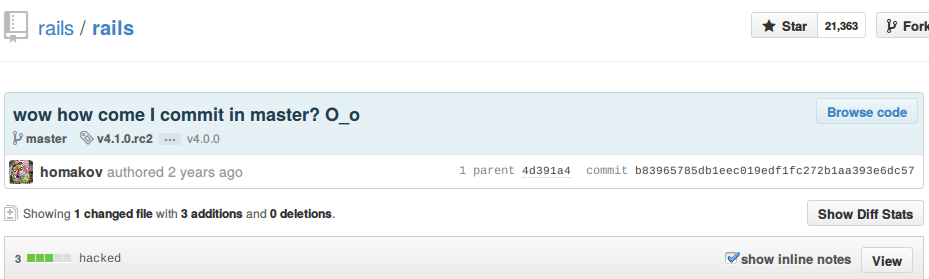
\includegraphics[width=\textwidth]{github-hack}
  \end{center}
  \pause
  You don't really control your project Git repository on GitHub.

  \pause
  Sometimes GitHub doesn't either.

  This is trust.
\end{frame}

\begin{frame}{}
  \centerline{\Huge I have issues with trust.}
\end{frame}

\begin{frame}{}
  Observation:

  \begin{center}
    \Large Free Software development and distribution relies on trust.
  \end{center}
\end{frame}

\begin{frame}{}
  Observation:

  \begin{center}
    \Large The Internet doesn't have a good, reliable, default way to
    facilitate trust.
  \end{center}
\end{frame}

\begin{frame}{}
  Problem:

  \begin{center}
    \Large We need a way to ensure the \textit{correctness} (i.e.,
    comes from the trusted source) and \textit{integrity} (i.e., was
    not modified between the trusted source and us) of arbitrary
    data.
  \end{center}
\end{frame}

\begin{frame}{}
  Solution:

  \begin{center}
    \Huge PGP.
  \end{center}
\end{frame}

\begin{frame}{What is PGP?}
  \begin{itemize}
  \item \textbf{P}retty \textbf{G}ood \textbf{P}rivacy
  \item Cf. OpenPGP, GPG (GnuPG)
  \item Technology for \textit{encrypting} and for \textit{signing}.
  \item Collectively I'll call these \textit{Crypto}.
  \end{itemize}
\end{frame}

\begin{frame}{What is PGP?}
  \textbf{Encryption}

  \begin{itemize}
  \item Obviously useful in certain cases.
  \item Personal communication: if I can, I encrypt.
  \item I won't be talking about it much.
    \begin{itemize}
    \item Free/Open Source Software projects are generally done out in
      the open.
    \item Encryption doesn't really help in this model.
    \end{itemize}
  \end{itemize}
\end{frame}

\begin{frame}{What is PGP?}
  \textbf{Signing}

  \begin{itemize}
    \item If Alice signs her message, Bob should be able to tell that:
      \begin{enumerate}
      \item It's from Alice, and no one else. (correctness \checkmark)
      \item It wasn't modified in transit, maliciously or
        otherwise. (integrity \checkmark)
      \end{enumerate}
    \item\textbf{PGP allows this.}
    \end{itemize}
\end{frame}

\begin{frame}{How can we trust PGP?}
  \begin{itemize}
    \item Uses \textit{public-key cryptography}.
    \item Remember that from CS2800?
      \begin{itemize}
      \item Boils down to the fact that it's really easy (polynomial
        time) to multiply two prime numbers, but really hard
        (exponential time) to factor the result back to those prime
        numbers.
      \item Especially when the numbers are very, very large.
      \item We can make a \textit{one-way function} that's fast to
        perform, but slow/practically impossible to undo.
      \item P=NP?
      \end{itemize}
    \item Cf. Shor's Algorithm, BQP time, $O\left((\log N)^3\right)$
      in $3N$ qubits to factor binary number $N$.
  \end{itemize}
\end{frame}

\begin{frame}{How can we trust PGP?}
  The algorithm:
  \begin{itemize}
  \item We have two prime numbers $p$ and $q$, and a number $N$ such
    that $N=pq$.
  \item We choose $d$,$e$ such that for any $A<N$,
    \begin{equation*}
      A = (A^e\operatorname{mod}N)^d\operatorname{mod}N
    \end{equation*}
  \item $M=(A^e\operatorname{mod}N)$ is our encrypted message.
  \item $A=(M^d\operatorname{mod}N)$ is our decrypted message.
  \item For messages larger than $N$, we either do it in blocks
    (encryption, guaranteed round-trip, but takes longer) or hash the
    message down to $<N$ bits (signing, depends on cryptographic
    security of hashing function).
  \end{itemize}
\end{frame}

\begin{frame}{How can we trust PGP?}
  We say the tuple $(e,N)$ is the \textit{public key}, and the tuple
  $(d,N)$ is the \textit{private key}.  We allow everyone to know the
  public key, but keep the private key hidden so that no one else
  knows it.

  This is common to all Public-Key Crypto: PGP, SSL/TLS, SSH, \dots
\end{frame}

\begin{frame}{How can we trust PGP?}
  \begin{center}
    \textbf{Encryption}
  \end{center}

  Anyone can encrypt to us
  \begin{equation*}
    M=A^e\operatorname{mod}N
  \end{equation*}
  but \textbf{only we can read it.}
  \begin{equation*}
    A=M^d\operatorname{mod}N
  \end{equation*}
\end{frame}

\begin{frame}{How can we trust PGP?}
  \begin{center}
    \textbf{Signature}:
  \end{center}

  \textbf{Only we can sign}
  \begin{equation*}
    S=A^d\operatorname{mod}N
  \end{equation*}
  but anyone can verify it
  \begin{equation*}
    A=S^e\operatorname{mod}N
  \end{equation*}
\end{frame}

\begin{frame}{How can we trust PGP?}
  \begin{center}
    \Large As long as the private key is held private, we can trust.
  \end{center}
\end{frame}

\begin{frame}{How do we use PGP?}
  We can sign any data we want to allow the user to verify:
  \begin{itemize}
  \item Debian, Fedora, etc packages
  \item Upstream release tarballs
  \item Release announcements
  \item Git tags
  \item Emails
  \item Git Commits (!)
  \item\dots?
  \end{itemize}
\end{frame}

\begin{frame}[fragile]{How do we use PGP?}
  For GNU/Linux, (technically OS X, Windows, too):
  
  \scriptsize
  \begin{lstlisting}
      # Generates a keypair
    $ gpg --gen-key
      # Generates a revocation certificate
    $ gpg -o revcert.asc --gen-revoke 12345ABC
      # Sign a file, makes filename.gpg
    $ gpg -s filename
      # Sign file in same file, makes filename.asc
    $ gpg --clearsign -a filename
      # Verify a signature or clearsigned message
    $ gpg --verify filename.asc
      # Encrypt a file, makes filename.gpg
    $ gpg -e filename
      # Decrypt a file and print its contents
    $ gpg --d filename.gpg
  \end{lstlisting}

  \normalsize
  Your mileage may vary (Debian, Ubuntu should use \texttt{gpg2},
  GPG4Win has graphical tool for making keys, etc).  Details on
  handout.
\end{frame}

\begin{frame}{}
  \centerline{\Huge Great!}
  
  \pause
  \centerline{\Large But wait...}
\end{frame}

\begin{frame}{}
  Problem:
  
  \begin{center}
    \Large How can we trust that the private key owner is who they
    say they are?
  \end{center}
\end{frame}

\begin{frame}{}
  Solution:

  \begin{center}
    \Huge Key Signing.
  \end{center}
\end{frame}

\begin{frame}{Key Signing}
  \begin{itemize}
  \item$\neq$ Crypto signing
  \item When you sign a key, you're saying that you have verified that
    the key belongs to the person it says.
  \item You need to know the key information (names, email addresses,
    comments, photos attached to the key).
  \item You need to know their personal information (from government
    issued photo ids, other documentation)
  \item Do they match?
  \item\textbf{Only sign what you have verified!  Only sign if you
      have verified!}
  \end{itemize}
\end{frame}

\begin{frame}{Key Signing}
  \begin{itemize}
  \item\textbf{Names:} Does the name on the key match the name on the
    photo ID?
    \pause
  \item\textbf{Emails:} Sign each email on the key separately,
    encrypted your signed key, and email that signed key to the
    email.  The key will be uploaded only if it can be decrypted
    (i.e., only if the key owner also controls the email account).
    \pause
  \item\textbf{Photo:} Does it match the photo ID and the person?
    (\textit{There isn't really a need for this, because it should
      already be verified by the name check.  Also, people's
      appearances change much more often than their names
      $\rightarrow$ less trust.})
    \pause
  \item\textbf{Comment:} Other documentation needed! (\textit{Again,
      seldom needed, because name verification should be sufficient.
      Also makes it much harder to establish trust.})
  \end{itemize}
\end{frame}

\begin{frame}{Key Signing}
  There's hidden trust in this!  You're trusting:
  \begin{itemize}
  \item Yourself, to follow this process.
    \pause
  \item The other person, to keep their private key secret.
    \pause
  \item The photo ID authority, to have verified this person's
    information. *
  \end{itemize}
  \pause

  A good rule of thumb is two photo IDs to verify, and more
  documentation if there is a comment.  One photo ID can be
  sufficient.  Use good judgment.
\end{frame}

\begin{frame}{}
  Problem:

  \begin{center}
    \Large I personally have to verify every single person I trust.
  \end{center}
\end{frame}

\begin{frame}{}
  Solution:

  \begin{center}
    \Huge Web of Trust
  \end{center}
\end{frame}

\begin{frame}{Web Of Trust (WoT)}
  \centerline{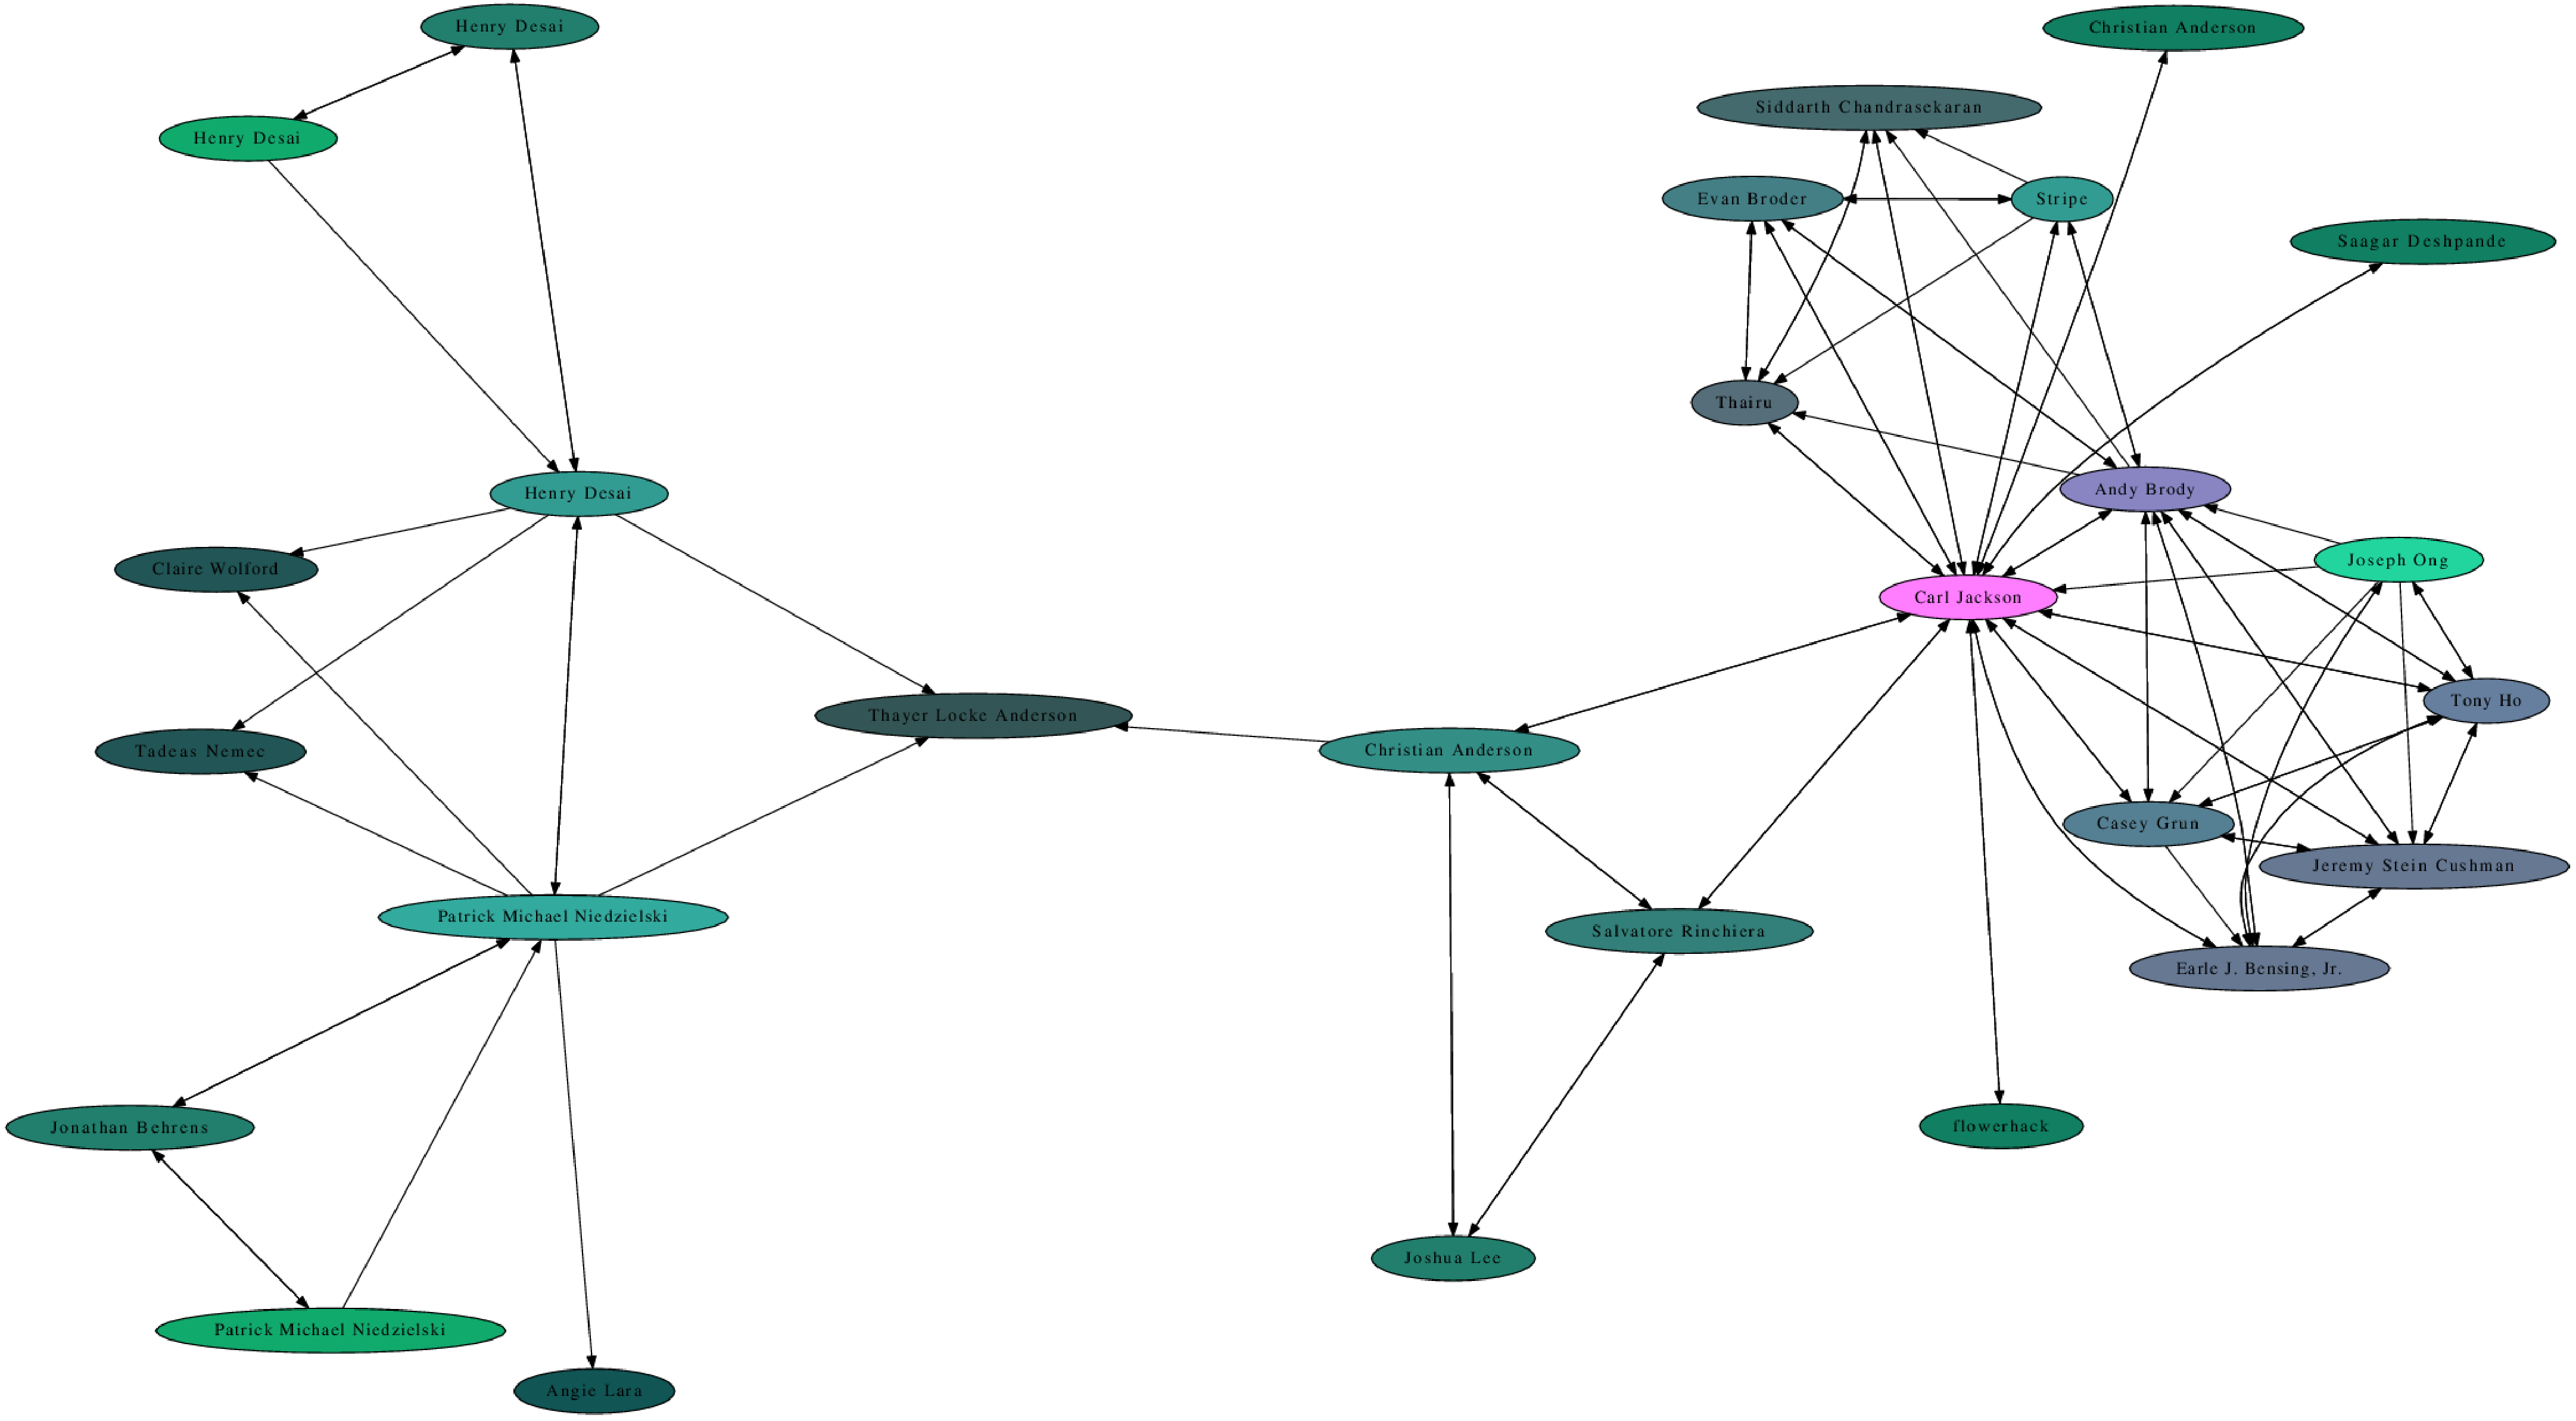
\includegraphics[width=0.75\textwidth]{wot}}
\end{frame}

\begin{frame}{Web Of Trust (WoT)}
  \begin{itemize}
  \item Alice signed Bob's key, and Bob signed Carol's key.  Why can't
    Alice trust Carol?
    \begin{itemize}
      \item She can, if she trusts that Bob followed the proper
        procedure in signing Carol's key.
      \item Trust both in the procedure and in others to follow the
        procedure.
    \end{itemize}
  \item Carol is said to be in Alice's \textit{web of trust}.
  \item\textbf{This is what distinguishes PGP from SSL/TLS and SSH.}
  \end{itemize}
\end{frame}

\begin{frame}{Web of Trust (WoT)}
  \begin{itemize}
  \item Maybe Bob seemed a little fishy.
  \item Let's add a \textit{trust level} to each key we know about:
    \begin{itemize}
    \item\textit{Untrusted}
    \item\textit{Marginal} (need two paths through marginal keys to trust a key)
    \item\textit{Complete} (need one path through complete key to
      trust a key)
    \item\textit{Ultimate} (you own the key)
    \end{itemize}
  \item This is not transitive, nor published!
    \begin{itemize}
    \item If Alice signed Bob, Bob signed Carol, and Carol signed
      Dave, then Alice needs to assign a trust level to Carol to trust
      Dave.
    \item If she doesn't know Carol, she can't trust Dave.
    \end{itemize}
  \item It's up to you whether you rely only on signature paths or on
    trust levels.  Signature paths give a bigger web of trust, but
    there's also a lot more trust involved!
  \end{itemize}
\end{frame}

\begin{frame}{Web of Trust (WoT)}
  \Large Expand your web of trust!
  \normalsize
  \begin{itemize}
  \item Have people sign your keys!
  \item Attend Cryptoparties (like this one!)
  \end{itemize}
\end{frame}

\begin{frame}{Recap}
  \begin{itemize}
  \item Trust is at the center of computer security, but also at the
    center of Free Software development.
  \item PGP gives us a way to formalize trust through Crypto and
    transform trust into true security.
  \item It does this by allowing us to sign keys we trust, associating
    people with keys.
  \item With a Web of Trust, we have far more people we can trust.
  \end{itemize}
\end{frame}

\begin{frame}{Questions?  Comments?}
  \begin{itemize}
  \item These slides (including source code) will be posted on my
    website following the talk.
  \item Cryptoparty!
    \begin{itemize}
    \item There are papers up at the front for setting up keys and
      signing others' keys on GNU/Linux and UNIX-y systems, OS X, and
      Windows.  Two sheets for each.
    \item If you need a key set up, ask on IRC or come talk to one of
      us.
    \item If you want to help set up keys, go for it!
    \item Sign keys!  Make sure you follow the keysigning procedure!
    \end{itemize}
  \item If you're interested in computer security or in the details of
    how PGP works, come up to me and chat.
  \end{itemize}
\end{frame}

\begin{frame}{Legal}
  \centerline{\ccby}
  \begin{center}
    Copyright \copyright{} 2014, Patrick M. Niedzielski. This work is
    released under the Creative Commons Attribution 4.0 United States
    License.
  \end{center}

  I give NO WARRANTEE to the validity or truth of the statements made
  within this presentation.  This presentation represent my views,
  plans, opinions, and ideas, not those of my employer, university, or
  any organizations to which I belong. The opinions expressed are
  solely my own.

  \medspace\medspace\medspace

  All of the images in this presentation I either created, have a
  license to use in this manner, am using under the United States Fair
  Use doctrine, or are trademarks which I use under U.S. Trademark
  law.  If you are the rights holder of any one of the images, and you
  believe that I do not have the rights to use that image, please
  contact me.
\end{frame}

\end{document}